\documentclass[../main.tex]{subfiles}
\usepackage{tikz}
\usepackage{physics}
\usepackage{amsmath}
\usepackage{tikz}
\usepackage{mathdots}
\usepackage{yhmath}
\usepackage{cancel}
\usepackage{color}
\usepackage{siunitx}
\usepackage{array}
\usepackage{multirow}
\usepackage{amssymb}
\usepackage{amsmath}
\usepackage{gensymb}
\usepackage{tabularx}
\usepackage{extarrows}
\usepackage{booktabs}
\usetikzlibrary{fadings}
\usetikzlibrary{patterns}
\usetikzlibrary{shadows.blur}
\usetikzlibrary{shapes}

\makeatletter
\renewcommand*\env@matrix[1][\arraystretch]{%
  \edef\arraystretch{#1}%
  \hskip -\arraycolsep
  \let\@ifnextchar\new@ifnextchar
  \array{*\c@MaxMatrixCols c}}
\makeatother

\begin{document}
    \tikzset{every picture/.style={line width=0.75pt}} %set default line width to 0.75pt        
    
    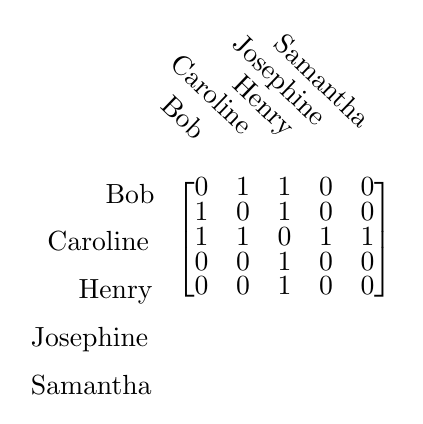
\begin{tikzpicture}[x=0.75pt,y=0.75pt,yscale=-1,xscale=1]
    %uncomment if require: \path (0,175); %set diagram left start at 0, and has height of 175
    
    % Text Node
    \draw (391,77) node [anchor=north west][inner sep=0.75pt]    {$\begin{bmatrix}[.7]
    0 & 1 & 1 & 0 & 0\\
    1 & 0 & 1 & 0 & 0\\
    1 & 1 & 0 & 1 & 1\\
    0 & 0 & 1 & 0 & 0\\
    0 & 0 & 1 & 0 & 0
    \end{bmatrix}$};
    % Text Node
    \draw (357,80) node [anchor=north west][inner sep=0.75pt]   [align=left] {Bob};
    % Text Node
    \draw (329,103) node [anchor=north west][inner sep=0.75pt]   [align=left] {Caroline};
    % Text Node
    \draw (344,126) node [anchor=north west][inner sep=0.75pt]   [align=left] {Henry};
    % Text Node
    \draw (321,149) node [anchor=north west][inner sep=0.75pt]   [align=left] {Josephine};
    % Text Node
    \draw (321,172) node [anchor=north west][inner sep=0.75pt]   [align=left] {Samantha};
    % Text Node
    \draw (390.54,35.74) node [anchor=north west][inner sep=0.75pt]  [rotate=-43.92] [align=left] {Bob};
    % Text Node
    \draw (395.06,15.74) node [anchor=north west][inner sep=0.75pt]  [rotate=-43.92] [align=left] {Caroline};
    % Text Node
    \draw (425.06,25.74) node [anchor=north west][inner sep=0.75pt]  [rotate=-43.92] [align=left] {Henry};
    % Text Node
    \draw (425.06,6.21) node [anchor=north west][inner sep=0.75pt]  [rotate=-43.92] [align=left] {Josephine};
    % Text Node
    \draw (445.06,6.21) node [anchor=north west][inner sep=0.75pt]  [rotate=-43.92] [align=left] {Samantha};
    \end{tikzpicture}
\end{document}